\chapter{Unterstützung nativer Komponenten in Ionic}
%
Cordova- und somit auch Ionic- Apps bieten die Möglichkeit native Funktionalitäten des jeweiligen Betriebssystems mittels Plugins zu erreichen. 

Ionic bietet eine ganze Reihe von eigenen nativen Komponenten (Ionic Native) an, die native Funktionalitäten ermöglichen und bereits mitgeliefert werden. Diese müssen lediglich aus der Bibliothek \texttt{ionic-native} importiert werden.

Ionic bietet zudem einen eigenen Vertriebsmarkt für Plugins an, in dem Entwickler ihre selbst geschriebenen Erweiterungen für Ionic entweder zum kostenfreien download unter einer Open Source Lizenz oder zum kostenpflichtigen verkauf anbieten können. 

Im folgenden soll eine sehr spezielle iOS- Funktionalität, nämlich die Unterstützung einer Kommunikation zwischen einer Ionic-App und einer Apple Watch gezeigt werden.
%
\section{Unterstützung von nativen Apple Watch Apps}
%
Im April 2015 hat Apple die Smart Watch Apple Watch veröffentlicht, die mit sogenannten WatchKit Apps erweitert werden kann. WatchKit Apps gehören jeweils zu einer iOS iPhone App und werden gemeinsam mit dem App-Bundle der iOS App ausgeliefert. Apple Watch Apps lassen sich zum jetzigen Zeitpunkt nicht mit Cordova realisieren, da Webviews für WatchKit Apps nicht Teil der API sind.
% https://developer.apple.com/watchos/
Zur Anbindung einer Apple Watch App an eine Cordova-App gibt es ein passendes Open Source Plugin \cite{CrossleyCordovaAppleWatchPlugin}, dessen Verwendung im Folgenden kurz erklärt wird.

Das Plugin liefert drei Arten der Kommunikation zwischen iPhone und Apple Watch:
\begin{itemize}
    \item \emph{Message passing:} Zweiseitige Übertragung von Strings oder JSON-Objekten zwischen Apple Watch- und Cordova-App.
    \item \emph{Local notifications:} Direktes Senden von Benachrichtigungen aus einer Cordova-App an die Apple Watch.
    \item \emph{User defaults:} Speichern von Daten, die sowohl von der Cordova- als auch von der Apple Watch-App zugänglich sind.
\end{itemize}
%
Der grundlegende Aufbau der Kommunikation zwischen Cordova- und Apple Watch-App ist in \fref{fig:watchPlugin} dargestellt. Das Plugin kommuniziert dabei mit einer iOS Bibliothek namens MMWormhole \cite{gitMMWormhole}. 
% https://github.com/20steps/cordova-plugin-watch
% https://github.com/mutualmobile/MMWormhole
% https://github.com/leecrossley/cordova-plugin-apple-watch#message-passing
% https://github.com/MobileChromeApps/cordova-plugin-background-app
%
\begin{figure}[!htb] 
	\centering
	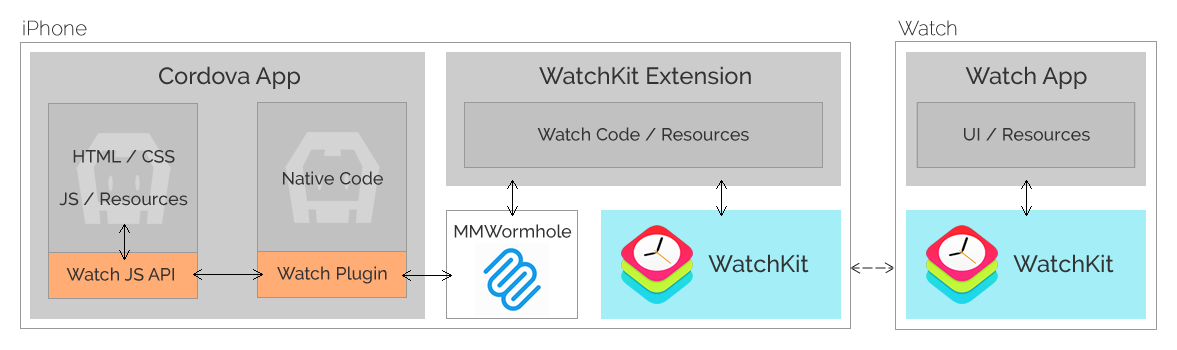
\includegraphics[width=0.9\textwidth]{data/bilder/apple-watch-plugin.png}
	\caption{Prinzip der Nachrichtenübermittlung mittels des Watch-Plugins \cite{CrossleyCordovaAppleWatchPlugin}}
	\label{fig:watchPlugin}
\end{figure}
%
MMWormhole erstellt dabei eine Art Brücke zwischen der App und ihrer Erweiterung mithilfe von App Groups, die Apple seit iOS 8 unterstützt. App Groups bieten mehreren Applikationen eines Entwicklers die Möglichkeit auf gemeinsame Daten zuzugreifen. So können auch Daten zwischen einer Extension und der eigentlichen iOS App ausgetauscht werden, was ansonsten aufgrund des Sandbox-Designs von iOS nicht möglich wäre.
%
% --------------------------------------------------------------------------------------------
%
\subsection{Grundsätzliche Methodik} 
%
\subsubsection{Ionic-Seite}
%
Zunächst muss eine Initialisierungsmethode \texttt{applewatch.init} aufgerufen werden:
\begin{lstlisting}[language=JavaScript]
applewatch.init(successHandler, errorHandler, appGroupId);
\end{lstlisting}
Dabei wird mittels des optionalen Parameters \texttt{appGroupId} die Application Group Id übergeben, die in XCode zunächst festgelegt werden muss. Dies führt zu einer Bindung zu der in XCode festgelegten Application Group.

Die Methode \texttt{applewatch.sendMessage} ermöglicht es nach erfolgreicher Initialisierung Strings oder JSON-Objekte an die Watch Extension zu senden. JSON-Objekte werden dabei automatisch in Strings umgewandelt.
\begin{lstlisting}[language=JavaScript]
applewatch.sendMessage(message, queueName, successHandler, errorHandler);
\end{lstlisting}
Der Parameter \texttt{queueName} muss dabei mit dem entsprechenden Listener der Watch App Funktion \texttt{MMWormhole.listenForMessageWithIdentifier} übereinstimmen. 

Mittels Listener-Funktionen auf Cordova-Seite können von der Apple Watch ausgesendete Nachrichten empfangen werden. Auch hier muss \texttt{queueName} mit der entsprechenden Methode auf Apple Watch Seite übereinstimmen.
\begin{lstlisting}[language=JavaScript]
applewatch.addListener(queueName, messageHandler);
applewatch.removeListener(queueName, successHandler, errorHandler);
\end{lstlisting}

Lokale Benachrichtigungen benötigen ebenfalls eine Registrierung. Es muss auf iOS Seite eine Erlaubnis gegeben werden, um lokale Nachrichten zu senden. Erfragt wird diese Erlaubnis mittels der Funktion \texttt{applewatch.registerNotifications}:
\begin{lstlisting}[language=JavaScript]
applewatch.registerNotifications(successHandler, errorHandler);
\end{lstlisting}
Wird die Erlaubnis durch den Nutzer erteilt, so wird der \texttt{successHandler} mit true aufgerufen. Sonst wird der \texttt{errorHandler} mit false aufgerufen.

Mithilfe der Funktion \texttt{applewatch.sendNotification} kann nun eine in einem JSON-Objekt (\texttt{payload}) gekapselte Nachricht an die Apple Watch gesendet werden.  
\begin{lstlisting}[language=JavaScript]
applewatch.sendNotification(successHandler, errorHandler, payload);
\end{lstlisting}
%
% --------------------------------------------------------------------------------------------
%
\subsubsection{Apple Watch-Seite}
Auf nativer Watchkit Extension Seite (hier beispielhaft in Swift) muss der Nachrichtenaustausch auch zunächst initialisiert werden:
\begin{lstlisting}[language=swift, breaklines=true]
let listeningSession = MMWormholeSession.sharedListeningSession();
listeningSession.activateSessionListening();

let wormhole = MMWormhole(applicationGroupIdentifier: "group.com.yourcompany", optionalDirectory: nil, transitingType: .SessionContext);
\end{lstlisting}

Die Methoden \texttt{passMessageObject} des MMWormhole- Objektes ermöglicht das Senden von Nachrichten. Mit Hilfe der Funktion \texttt{listenForMessageWithIdentifier} des MMWormholeSession-Objektes kann ein Listener erstellt werden:
\begin{lstlisting}[language=swift, breaklines=true]
wormhole.passMessageObject("titleString", identifier: "queueName");

listeningSession.listenForMessageWithIdentifier("queueName", listener: { (messageObject) -> Void in
    if let message: AnyObject = messageObject {
        // Do something
    }
});
\end{lstlisting}
%
% --------------------------------------------------------------------------------------------
%
\subsection{Skizzierung einer möglichen Anwendung bei einer Tagungsapp}
%
Gegeben sei eine App, in der Inhalte einer Tagung oder Messe dargestellt werden können. Diese App ist vollständig in Ionic geschrieben. Als Datenpersistierung wird eine Web SQL Datenbank verwendet. Diese wird gewrappt mit einer asynchronen objekt-relationalen JavaScript Mapper namens \emph{persistenceJS}, der auf dem Cordova SQLite Plugin aufbaut. In der Tagungsapp werden unter anderem Listen von Vorträgen und Diskussionsbeiträgen mit ihren Detailinformationen aufgelistet. Nutzer können dabei einzelne Beiträge als Favoriten markieren. Zudem können sich einzelne Teilnehmer mit Teilnehmern und Ausstellern verabreden.

In einer möglichen zugehörigen Apple Watch Companion-App sollen ausgewählte Inhalte wie Favorisierte Vorträge oder die Terminabsprachen auf der Watch-App aufgeführt werden. Zu gegebener Zeit soll der Nutzer zudem über ein Notificationsystem innerhalb der Apple Watch an die Termine erinnert werden können.

Dazu muss der Datenaustausch zwischen 